\documentclass[11pt,a4paper]{article}

% --- Essential Typographic & Layout Packages ---
\usepackage[utf8]{inputenc}
\usepackage[T1]{fontenc}
\usepackage[margin=1in]{geometry} % Professional page margins
\usepackage{microtype}            % Subliminal typographic micro-adjustments
\usepackage{amsmath,amsfonts}     % Advanced math typesetting
\usepackage{ulem}                 % Needed for strike-through (\sout)
\usepackage{enumitem}             % Customized lists without ugly gaps

% --- Color & UI Background Packages ---
\usepackage[dvipsnames]{xcolor}
\usepackage[most]{tcolorbox}      % For premium callout boxes / backgrounds

% --- Design Palette Definition ---
\definecolor{DeepNavy}{RGB}{24, 43, 73}
\definecolor{AccentBlue}{RGB}{54, 95, 145}
\definecolor{LightBg}{RGB}{245, 247, 250}
\definecolor{BorderGray}{RGB}{218, 224, 233}

% --- Custom Header Formatting ---
\newcommand{\Heading}[1]{\vspace{0.4cm}\noindent\textbf{\textcolor{DeepNavy}{\large #1}}\par\vspace{0.15cm}}

\begin{document}

% --- Title Section ---
\begin{center}
    {\LARGE\bfseries\textcolor{DeepNavy}{Advanced Calculus}}
    \vspace{0.6cm}
\end{center}

\Heading{Differential Equations (DE):}
An equation involving derivatives of one or more dependent variables with respect to one or more independent variables is called a differential equation.

\Heading{Ordinary Differential Equations (ODE):}
A differential equation involving ordinary derivatives of one or more dependent variables with respect to a single independent variable is called an ordinary differential equation.

\Heading{Partial Differential Equation (PDE):}
A differential equation involving partial derivatives of one or more dependent variables with respect to more than one independent variable is called a partial differential equation.

% --- Stylized Background Callout for Examples ---
\begin{tcolorbox}[colback=LightBg, colframe=BorderGray, arc=4mm]
    {\small\textbf{\textcolor{AccentBlue}{EXAMPLES BY CATEGORY}}}
    \vspace{0.2cm}
    \begin{description}[leftmargin=0.4cm, style=nextline, font=\normalfont\bfseries\textcolor{DeepNavy}]
        
        \item[Ordinary Differential Equations (ODE)]
        \[ \frac{d^2y}{dx^2} + xy\left(\frac{dy}{dx}\right)^2 = 0 \]
        \[ \frac{d^4x}{dt^4} + 5\frac{d^2x}{dt^2} + 3x = \sin(t) \]
        
        \item[Partial Differential Equations (PDE)]
        \[ \frac{\partial v}{\partial \sigma} + \frac{\partial v}{\partial t} = v \]
        \[ \frac{\partial^2u}{\partial x^2} + \frac{\partial^2u}{\partial y^2} + \frac{\partial^2u}{\partial z^2} = 0 \]
        
        \item[Not DE but Basic Derivatives]
        \[ \frac{d}{dx}\left(e^{ax}\right) = ae^{ax} \]
        \[ \frac{d}{dx}(uv) = u\frac{dv}{dx} + v\frac{du}{dx} \]
        
    \end{description}
\end{tcolorbox}

\Heading{Order of a DE:}
The order of the highest-order derivative involved in a differential equation is called the order of the differential equation.

\Heading{Degree of a DE:}
The degree of a differential equation is the power of the highest-order derivative present in the equation.

\begin{tcolorbox}[colback=LightBg, colframe=BorderGray, arc=4mm]
    {\small\textbf{\textcolor{AccentBlue}{EXAMPLES BY CATEGORY}}}
    \vspace{0.2cm}
    \begin{description}[leftmargin=0.4cm, style=nextline, font=\normalfont\bfseries\textcolor{DeepNavy}]
        \item[1st Order 1st Degree ODE]
        \[ \frac{dy}{dx} + y = e^x \]
        
        \item[2nd Order 1st Degree ODE]
        \[ \frac{d^2y}{dx^2} + 3\frac{dy}{dx} + 2y = 0 \]
        
        \item[2nd Order 2nd Degree ODE]
        \[ \left(\frac{d^2y}{dx^2}\right)^2 + y\frac{dy}{dx} = 0 \]
        
        \item[1st Order 1st Degree PDE]
        \[ \frac{\partial u}{\partial t} + \frac{\partial u}{\partial x} = 0 \]
        
        \item[2nd Order 1st Degree PDE]
        \[ \frac{\partial^2 u}{\partial t^2} - c^2 \frac{\partial^2 u}{\partial x^2} = 0 \]
        
        \item[2nd Order 2nd Degree PDE]
        \[ \left(\frac{\partial^2 u}{\partial x^2}\right)^2 + \left(\frac{\partial^2 u}{\partial y^2}\right)^2 = 0 \]
    \end{description}
\end{tcolorbox}

\Heading{Linear ODE:}
A linear ordinary differential equation of order $n$, in the dependent variable $y$ and the independent variable $x$, is an equation that can be expressed in the form.
\[
a_0 y^{(n)} + a_1 y^{(n-1)} + \ldots + a_n y = f(x)
\]
or equivalently,
\[
a_0(x) \frac{d^n y}{dx^n} + a_1(x) \frac{d^{n-1} y}{dx^{n-1}} + \ldots + a_n(x) y = f(x)
\]
where $a_0, a_1, \ldots, a_n$ are functions of $x$ (not identically zero) and $f(x)$ is a given function.

\vspace{0.2cm}
\noindent\textbf{\textcolor{DeepNavy}{Important Observations:}}
\begin{enumerate}[label=\arabic*), leftmargin=0.6cm, itemsep=0.05cm]
    \item The dependent variable $y$ and its various derivatives occur to the first degree only.
    \item No products of $y$ and/or any of its derivatives are present.
    \item No transcendental functions of $y$ or its derivatives occur (e.g., $\sin y$, $e^y$).
\end{enumerate}

\Heading{Nonlinear ODE:}
A nonlinear ordinary differential equation is an ordinary differential equation that is not linear.

\begin{tcolorbox}[colback=LightBg, colframe=BorderGray, arc=4mm]
    {\small\textbf{\textcolor{AccentBlue}{EXAMPLES BY CATEGORY}}}
    \vspace{0.2cm}
    \begin{description}[leftmargin=0.4cm, style=nextline, font=\normalfont\bfseries\textcolor{DeepNavy}]
        \item[Linear ODE with Constant Coefficients]
        \[ \frac{d^2y}{dx^2} + 3\frac{dy}{dx} + 2y = 0 \]
        
        \item[Linear ODE with Variable Coefficients]
        \[ \frac{d^4y}{dx^4} + x^{30}\frac{dy}{dx} + 2y = xe^x \]
        
        \item[Nonlinear ODE Examples]
        \[ \left(\frac{d^2y}{dx^2}\right)^2 + y\frac{dy}{dx} = 0 \]
        \[ \frac{dy}{dx} + \sin(y) = 0 \] % Replaced the incorrect linear equation with a proper nonlinear one
        \[ A \frac{d^2y}{dx^2} + K \frac{d^3y}{dx^3} + x \frac{dy}{dx} = x e^x \frac{dx}{dy} \]
        
        \item[General Form of a Nonlinear ODE]
        \[ F\left(x, y, \frac{dy}{dx}, \frac{d^2y}{dx^2}, \ldots, \frac{d^ny}{dx^n}\right) = 0 \]
    \end{description}
\end{tcolorbox}

\Heading{What Makes an ODE Nonlinear?}
An ODE is classified as nonlinear if it violates any of the key linear criteria:
\begin{itemize}[leftmargin=0.5cm, itemsep=0.05cm]
    \item \textbf{Higher Powers:} Any $y$ or derivative term has an exponent other than 1.
    \item \textbf{Product Terms:} The variable $y$ is multiplied by its own derivatives.
    \item \textbf{Nonlinear Functions:} The equation contains functions like $\sin(y)$, $e^{y}$, or $\ln(y)$.
\end{itemize}

\Heading{Origin and Application:}
Differential equations occur in connection with numerous problems encountered across various branches of science and engineering:
\begin{itemize}[leftmargin=0.5cm, itemsep=0.05cm]
    \item Population Dynamics
    \item Dynamical Systems and Chaos
    \item Fluid Dynamics
    \item Heterogeneous Heat Transfer
    \item Biophysics and Mathematical Biology
\end{itemize}

\Heading{Formation of Differential Equations:}
To form a differential equation from a given relation involving independent/dependent variables and arbitrary constants, we eliminate the arbitrary constants by successive differentiation.

\noindent\textbf{Example Problem:} \\
Form the differential equation by eliminating the constants $a$ and $b$ from:
\begin{equation}
    y = ax + bx^2
\end{equation}

\noindent\textbf{Solution:} \\
Given the relation with two arbitrary constants $a$ and $b$:
\begin{equation}
    y = ax + bx^2 \label{eq:original}
\end{equation}

Since there are two arbitrary constants, we differentiate the equation twice with respect to $x$ to eliminate them.

\paragraph{Step 1: First Differentiation}
Differentiating Equation \eqref{eq:original} with respect to $x$:
\begin{equation}
    \frac{dy}{dx} = a + 2bx \label{eq:diff1}
\end{equation}

\paragraph{Step 2: Second Differentiation}
Differentiating Equation \eqref{eq:diff1} with respect to $x$:
\begin{equation}
    \frac{d^2y}{dx^2} = 2b \implies b = \frac{1}{2}\frac{d^2y}{dx^2} \label{eq:b_val}
\end{equation}

\paragraph{Step 3: Eliminate Constant $a$}
Substitute the value of $b$ from Equation \eqref{eq:b_val} into Equation \eqref{eq:diff1}:
\[
\frac{dy}{dx} = a + 2\left(\frac{1}{2}\frac{d^2y}{dx^2}\right)x
\]
\[
\frac{dy}{dx} = a + x\frac{d^2y}{dx^2} \implies a = \frac{dy}{dx} - x\frac{d^2y}{dx^2} \label{eq:a_val}
\]

\paragraph{Step 4: Substitute $a$ and $b$ into the Original Equation}
Substitute the expressions for $a$ and $b$ back into Equation \eqref{eq:original}:
\[
y = \left(\frac{dy}{dx} - x\frac{d^2y}{dx^2}\right)x + \left(\frac{1}{2}\frac{d^2y}{dx^2}\right)x^2
\]
Expand the terms:
\[
y = x\frac{dy}{dx} - x^2\frac{d^2y}{dx^2} + \frac{1}{2}x^2\frac{d^2y}{dx^2}
\]
Combine the like terms of $\frac{d^2y}{dx^2}$:
\[
y = x\frac{dy}{dx} - \frac{1}{2}x^2\frac{d^2y}{dx^2}
\]

\paragraph{Final Form:}
Multiply the entire equation by $2$ and rearrange terms to obtain the standard form:
\begin{equation}
    x^2\frac{d^2y}{dx^2} - 2x\frac{dy}{dx} + 2y = 0
\end{equation}
This is the required ordinary differential equation of \text{$2^{nd}$ order and $1^{st}$ degree.}



\section{Equations Reducible to Homogeneous Form}
A differential equation of the form
\[ \frac{dy}{dx} = \frac{ax+by+c}{a_1x+b_1y+c_1}, \quad \text{where } \frac{a}{a_1} \neq \frac{b}{b_1} \]
can be reduced to a homogeneous form by putting $x = X+h$ and $y = Y+k$. Then, $\frac{dY}{dX} = \frac{dy}{dx}$.

\begin{tcolorbox}[colback=LightBg, colframe=BorderGray, arc=4mm]
    {\small\textbf{\textcolor{AccentBlue}{EXAMPLE: REDUCIBLE TO HOMOGENEOUS FORM}}}
    \vspace{0.2cm}\\
    \textbf{Solve:} $\displaystyle \frac{dy}{dx} = \frac{x+2y-3}{2x+y-3}$ \hfill (1)
    
    \vspace{0.2cm}
    \textbf{Solution:} \\
    Put $x = X+h$ and $y = Y+k$, where $h$ and $k$ are constants. \\
    Then, $\frac{dy}{dx} = \frac{dY}{dX}$. \\
    Substituting into (1):
    \[ \frac{dY}{dX} = \frac{X+h+2(Y+k)-3}{2(X+h)+(Y+k)-3} = \frac{X+2Y + (h+2k-3)}{2X+Y + (2h+k-3)} \]
    Now, choose $h$ and $k$ so that:
    \[ h+2k-3 = 0 \quad \text{and} \quad 2h+k-3 = 0 \]
    Solving these equations, we get $h=1$ and $k=1$. \\
    Therefore, the equation becomes:
    \[ \frac{dY}{dX} = \frac{X+2Y}{2X+Y} \]
    which is homogeneous in $X$ and $Y$. \\
    Put $Y = vX$, so that $\frac{dY}{dX} = v + X\frac{dv}{dX}$.
    \[ v + X\frac{dv}{dX} = \frac{X+2vX}{2X+vX} = \frac{1+2v}{2+v} \]
    \[ X\frac{dv}{dX} = \frac{1+2v}{2+v} - v = \frac{1+2v-2v-v^2}{2+v} = \frac{1-v^2}{2+v} \]
    Separating the variables:
    \[ \frac{dX}{X} = \left(\frac{2+v}{1-v^2}\right)dv = \left(\frac{2}{1-v^2} + \frac{v}{1-v^2}\right)dv \]
    Integrating both sides:
    \[ \ln X = 2 \cdot \frac{1}{2} \ln \left(\frac{1+v}{1-v}\right) - \frac{1}{2} \ln(1-v^2) + \ln c \]
    \[ \Rightarrow X = c \left( \frac{1+v}{1-v} \cdot \frac{1}{\sqrt{1-v^2}} \right) = c \left( \frac{1+v}{1-v} \cdot \frac{1}{\sqrt{1+v}\sqrt{1-v}} \right) \]
    \[ \Rightarrow X = \frac{c\sqrt{1+v}}{(1-v)^{3/2}} \]
    Squaring both sides:
    \[ X^2 = \frac{c^2(1+v)}{(1-v)^3} \implies X^2 (1-v)^3 = c^2 (1+v) \]
    Substituting $v = \frac{Y}{X}$:
    \[ X^2 \left(1 - \frac{Y}{X}\right)^3 = c^2 \left(1 + \frac{Y}{X}\right) \]
    \[ \Rightarrow X^2 \frac{(X-Y)^3}{X^3} = c^2 \left(\frac{X+Y}{X}\right) \implies (X-Y)^3 = c^2(X+Y) \]
    Finally, substituting back $X = x-1$ and $Y = y-1$:
    \[ \{ (x-1) - (y-1) \}^3 = c^2 \{ (x-1) + (y-1) \} \]
    \[ \Rightarrow (x-y)^3 = c^2 (x+y-2) \]
    which is the required solution.
\end{tcolorbox}

\section{Linear Differential Equations}
A differential equation of the form
\[ \frac{dy}{dx} + P(x)y = Q(x) \]
is called a linear differential equation of the first order.

\vspace{0.2cm}
\noindent\textbf{\textcolor{DeepNavy}{Method of Solution:}} \\
To solve the equation $\frac{dy}{dx} + P(x)y = Q(x)$ (1), we multiply both sides by an \textbf{Integrating Factor (I.F.)}. \\
The Integrating Factor is given by $e^{\int P(x)dx}$. \\
Multiplying (1) by the I.F.:
\[ e^{\int P(x)dx} \frac{dy}{dx} + P(x)y e^{\int P(x)dx} = Q(x)e^{\int P(x)dx} \]
Notice that the left-hand side is the exact derivative of the product $y \cdot e^{\int P(x)dx}$:
\[ \frac{d}{dx} \left( y e^{\int P(x)dx} \right) = Q(x) e^{\int P(x)dx} \]
Integrating with respect to $x$:
\[ y e^{\int P(x)dx} = \int Q(x) e^{\int P(x)dx} dx + c \]
which is the required general solution.

\begin{tcolorbox}[colback=LightBg, colframe=BorderGray, arc=4mm]
    {\small\textbf{\textcolor{AccentBlue}{EXAMPLE: LINEAR DE}}}
    \vspace{0.2cm}\\
    \textbf{Solve:} $\displaystyle x\frac{dy}{dx} + 2y = x^2\log x$ \hfill (1)
    
    \vspace{0.2cm}
    \textbf{Solution:} \\
    Dividing by $x$, we put the equation in standard linear form:
    \[ \frac{dy}{dx} + \frac{2}{x}y = x \log x \]
    Here, $P(x) = \frac{2}{x}$ and $Q(x) = x \log x$. \\
    The Integrating Factor (I.F.) is:
    \[ \text{I.F.} = e^{\int \frac{2}{x}dx} = e^{2\log x} = e^{\log x^2} = x^2 \]
    Multiplying both sides of the standard equation by $x^2$:
    \[ x^2\frac{dy}{dx} + 2xy = x^3\log x \]
    \[ \Rightarrow \frac{d}{dx} (y x^2) = x^3 \log x \]
    Integrating both sides:
    \[ x^2 y = \int x^3 \log x \, dx + c \]
    Using integration by parts (taking $\log x$ as the first function and $x^3$ as the second):
    \[ x^2 y = \log x \cdot \frac{x^4}{4} - \int \frac{1}{x} \cdot \frac{x^4}{4} dx + c \]
    \[ \Rightarrow x^2 y = \frac{x^4}{4} \log x - \frac{1}{4} \int x^3 dx + c \]
    \[ \Rightarrow x^2 y = \frac{x^4}{4} \log x - \frac{1}{4} \cdot \frac{x^4}{4} + c = \frac{x^4}{4} \left(\log x - \frac{1}{4}\right) + c \]
    Dividing by $x^2$:
    \[ y = cx^{-2} + \frac{1}{4} x^2 \left(\log x - \frac{1}{4}\right) \]
    which is the required solution.
\end{tcolorbox}

\begin{tcolorbox}[colback=LightBg, colframe=BorderGray, arc=4mm]
    {\small\textbf{\textcolor{AccentBlue}{EXAMPLE: INITIAL VALUE PROBLEM (IVP)}}}
    \vspace{0.2cm}\\
    \textbf{Solve the IVP:} $\displaystyle (x^2+1)\frac{dy}{dx} + 4xy = x, \quad y(2)=1$ \hfill (2)
    
    \vspace{0.2cm}
    \textbf{Solution:} \\
    Dividing by $(x^2+1)$, we obtain the standard linear form:
    \[ \frac{dy}{dx} + \frac{4x}{x^2+1}y = \frac{x}{x^2+1} \hfill (3) \]
    Here, $P(x) = \frac{4x}{x^2+1}$. The Integrating Factor is:
    \[ \text{I.F.} = e^{\int \frac{4x}{x^2+1} dx} = e^{2\ln(x^2+1)} = e^{\ln((x^2+1)^2)} = (x^2+1)^2 \]
    Multiplying equation (3) by the I.F.:
    \[ (x^2+1)^2 \frac{dy}{dx} + \frac{4x}{x^2+1}(x^2+1)^2 y = \frac{x}{x^2+1}(x^2+1)^2 \]
    \[ \Rightarrow (x^2+1)^2 \frac{dy}{dx} + 4x(x^2+1)y = x(x^2+1) \]
    \[ \Rightarrow \frac{d}{dx} \left( (x^2+1)^2 y \right) = x^3 + x \]
    Integrating both sides:
    \[ (x^2+1)^2 y = \int (x^3 + x) dx + c \]
    \[ \Rightarrow (x^2+1)^2 y = \frac{x^4}{4} + \frac{x^2}{2} + c \hfill (4) \]
    Applying the initial condition $y(2)=1$ (i.e., when $x=2, y=1$):
    \[ (2^2+1)^2 \cdot 1 = \frac{2^4}{4} + \frac{2^2}{2} + c \implies 5^2 = \frac{16}{4} + \frac{4}{2} + c \]
    \[ 25 = 4 + 2 + c \implies c = 19 \]
    Substituting $c=19$ back into equation (4):
    \[ (x^2+1)^2 y = \frac{x^4}{4} + \frac{x^2}{2} + 19 \]
    This is the required solution.
\end{tcolorbox}

\section{Bernoulli Equations}
A differential equation of the form
\[ \frac{dy}{dx} + P(x)y = Q(x)y^n \hfill (1) \]
is called a Bernoulli differential equation.

\vspace{0.2cm}
\noindent\textbf{\textcolor{DeepNavy}{Method of Solution:}} \\
Divide equation (1) by $y^n$:
\[ y^{-n}\frac{dy}{dx} + P(x)y^{-n+1} = Q(x) \hfill (2) \]
Put $y^{-n+1} = v$. Then differentiating with respect to $x$:
\[ (-n+1)y^{-n}\frac{dy}{dx} = \frac{dv}{dx} \implies y^{-n}\frac{dy}{dx} = \frac{1}{1-n}\frac{dv}{dx} \]
Substitute this into equation (2):
\[ \frac{1}{1-n}\frac{dv}{dx} + P(x)v = Q(x) \]
\[ \Rightarrow \frac{dv}{dx} + (1-n)P(x)v = (1-n)Q(x) \]
This is a linear differential equation in $v$ and $x$, which can be solved using the integrating factor method.

\vspace{0.2cm}
\noindent\textbf{\textcolor{DeepNavy}{General Case:}} \\
An equation of the form $f'(y)\frac{dy}{dx} + P(x)f(y) = Q(x)$ can be reduced to a linear form by putting $f(y) = v$, which gives $f'(y)\frac{dy}{dx} = \frac{dv}{dx}$. The equation becomes:
\[ \frac{dv}{dx} + P(x)v = Q(x) \]
which is linear in $v$ and $x$.

\begin{tcolorbox}[colback=LightBg, colframe=BorderGray, arc=4mm]
    {\small\textbf{\textcolor{AccentBlue}{EXAMPLE: BERNOULLI EQUATION}}}
    \vspace{0.2cm}\\
    \textbf{Solve:} $\displaystyle \frac{dy}{dx} + y = xy^3$ \hfill (1)
    
    \vspace{0.2cm}
    \textbf{Solution:} \\
    This is a Bernoulli differential equation with $n=3$. Dividing by $y^3$:
    \[ y^{-3}\frac{dy}{dx} + y^{-2} = x \]
    Let $v = y^{1-n} = y^{1-3} = y^{-2}$. Then differentiating with respect to $x$:
    \[ \frac{dv}{dx} = -2y^{-3}\frac{dy}{dx} \implies y^{-3}\frac{dy}{dx} = -\frac{1}{2}\frac{dv}{dx} \]
    Substitute this back into the equation:
    \[ -\frac{1}{2}\frac{dv}{dx} + v = x \implies \frac{dv}{dx} - 2v = -2x \hfill (2) \]
    This is a linear differential equation in $v$ and $x$. Here, $P(x) = -2$. \\
    The Integrating Factor is:
    \[ \text{I.F.} = e^{\int -2 dx} = e^{-2x} \]
    Multiplying equation (2) by the I.F.:
    \[ e^{-2x}\frac{dv}{dx} - 2v e^{-2x} = -2x e^{-2x} \]
    \[ \Rightarrow \frac{d}{dx} \left( v e^{-2x} \right) = -2x e^{-2x} \]
    Integrating both sides:
    \[ v e^{-2x} = \int -2x e^{-2x} dx + c \]
    Using integration by parts:
    \[ v e^{-2x} = -2 \left[ x\left(\frac{e^{-2x}}{-2}\right) - \int 1 \cdot \left(\frac{e^{-2x}}{-2}\right) dx \right] + c \]
    \[ v e^{-2x} = x e^{-2x} - \int e^{-2x} dx + c = x e^{-2x} + \frac{1}{2} e^{-2x} + c \]
    Dividing by $e^{-2x}$:
    \[ v = x + \frac{1}{2} + c e^{2x} \]
    where $c$ is an arbitrary constant. \\
    Since $v = y^{-2} = \frac{1}{y^2}$, we obtain the solution in the form:
    \[ \frac{1}{y^2} = x + \frac{1}{2} + c e^{2x} \]
\end{tcolorbox}

\begin{tcolorbox}[colback=LightBg, colframe=BorderGray, arc=4mm]
    {\small\textbf{\textcolor{AccentBlue}{EXAMPLE: BERNOULLI EQUATION}}}
    \vspace{0.2cm}\\
    \textbf{Solve:} $\displaystyle x\frac{dy}{dx} + y = y^2 \log x$ \hfill (1)
    
    \vspace{0.2cm}
    \textbf{Solution:} \\
    Dividing by $xy^2$:
    \[ \frac{1}{x}y^{-2}\frac{dy}{dx} + \frac{1}{x}y^{-1} = \frac{1}{x}\log x \]
    Actually, dividing the whole equation by $y^2$ first and then dividing the whole equation by $x$:
    \[ y^{-2}\frac{dy}{dx} + \frac{1}{x}y^{-1} = \frac{1}{x}\log x \]
    Put $-y^{-1} = v \implies y^{-2}\frac{dy}{dx} = \frac{dv}{dx}$. \\
    Substitute into the equation:
    \[ \frac{dv}{dx} - \frac{1}{x}v = \frac{1}{x}\log x \hfill (2) \]
    The Integrating Factor is:
    \[ \text{I.F.} = e^{\int -\frac{1}{x} dx} = e^{-\log x} = \frac{1}{x} \]
    Multiplying equation (2) by the I.F.:
    \[ \frac{1}{x}\frac{dv}{dx} - \frac{1}{x^2}v = \frac{1}{x^2}\log x \]
    \[ \Rightarrow \frac{d}{dx} \left( v \cdot \frac{1}{x} \right) = \frac{1}{x^2}\log x \]
    Integrating both sides:
    \[ v \cdot \frac{1}{x} = \int \frac{1}{x^2}\log x \, dx + c \]
    Using integration by parts:
    \[ \int x^{-2}\log x \, dx = \log x \left(\frac{x^{-1}}{-1}\right) - \int \frac{1}{x} \left(\frac{x^{-1}}{-1}\right) dx \]
    \[ = -\frac{1}{x}\log x + \int x^{-2} dx = -\frac{1}{x}\log x - \frac{1}{x} \]
    So we have:
    \[ \frac{v}{x} = c - \frac{1}{x}\log x - \frac{1}{x} = c - \frac{1 + \log x}{x} \]
    Multiplying by $x$:
    \[ v = cx - (1 + \log x) \]
    Since $v = -y^{-1} = -\frac{1}{y}$:
    \[ -\frac{1}{y} = cx - (1 + \log x) \implies \frac{1}{y} = (1 + \log x) - cx \]
    This is the required solution.
\end{tcolorbox}

\section{Exact Differential Equations}

\textbf{\textcolor{DeepNavy}{Total Differential:}} \\
If the function $F(x,y)$ has continuous first partial derivatives in a domain $D$, then the total differential $dF$ is defined by:
\[ dF(x,y) = \frac{\partial F(x,y)}{\partial x}dx + \frac{\partial F(x,y)}{\partial y}dy \quad \forall (x,y) \in D \]

\textbf{\textcolor{DeepNavy}{Exact Differential:}} \\
The expression $M(x,y)dx + N(x,y)dy$ is called an exact differential if there exists a function $F(x,y)$ such that:
\[ dF(x,y) = M(x,y)dx + N(x,y)dy \]

\textbf{\textcolor{DeepNavy}{Theorem (Necessary Condition):}} \\
Consider the DE $M(x,y)dx + N(x,y)dy = 0$ where $M(x,y)$ and $N(x,y)$ have continuous $1^{\text{st}}$ partial derivatives $\forall (x,y) \in D$. \\
If the DE (1) is exact in $D$, then $\frac{\partial M(x,y)}{\partial y} = \frac{\partial N(x,y)}{\partial x} \quad \forall (x,y) \in D$.

Conversely, if $\frac{\partial M(x,y)}{\partial y} = \frac{\partial N(x,y)}{\partial x} \quad \forall (x,y) \in D$, then the DE (1) is exact in $D$.

\vspace{0.2cm}
\noindent\textbf{\textcolor{DeepNavy}{Working Rule:}} \\
If the DE $M(x,y)dx + N(x,y)dy = 0$ satisfies the condition $\frac{\partial M}{\partial y} = \frac{\partial N}{\partial x}$, then it is exact. \\
To integrate it:
\begin{enumerate}
    \item Integrate $M$ with respect to $x$ regarding $y$ as a constant.
    \item Find out those terms in $N$ which are free from $x$ and integrate them with respect to $y$.
    \item Add the two expressions so obtained and equate the sum to an arbitrary constant.
\end{enumerate}
This gives the general solution of the given exact DE.

\begin{tcolorbox}[colback=LightBg, colframe=BorderGray, arc=4mm]
    {\small\textbf{\textcolor{AccentBlue}{EXAMPLE: EXACT DE}}}
    \vspace{0.2cm}\\
    \textbf{Solve:} $\displaystyle (3x^2 + 4xy)dx + (2x^2 + 2y)dy = 0$
    
    \vspace{0.2cm}
    \textbf{Solution:} \\
    Here, $M(x,y) = 3x^2 + 4xy$ and $N(x,y) = 2x^2 + 2y$.
    \[ \frac{\partial M}{\partial y} = 4x \quad \text{and} \quad \frac{\partial N}{\partial x} = 4x \]
    Since $\frac{\partial M}{\partial y} = \frac{\partial N}{\partial x}$, the given equation is exact in every rectangular domain $D$.
    
    According to the working rule:
    \begin{enumerate}
        \item Integrate $M$ with respect to $x$ regarding $y$ as a constant:
        \[ \int M(x,y) dx = \int (3x^2 + 4xy) dx = x^3 + 2x^2y \]
        \item The terms in $N(x,y)$ free from $x$ are $2y$. Integrate this with respect to $y$:
        \[ \int 2y \, dy = y^2 \]
    \end{enumerate}
    Adding these two and equating to a constant:
    \[ x^3 + 2x^2y + y^2 = c \]
    which is the required solution. \\
    \textbf{Note:} You may solve it as it's given in J.L. Ross.
\end{tcolorbox}

\begin{tcolorbox}[colback=LightBg, colframe=BorderGray, arc=4mm]
    {\small\textbf{\textcolor{AccentBlue}{EXAMPLE: EXACT DE (IVP)}}}
    \vspace{0.2cm}\\
    \textbf{Solve the IVP:} $\displaystyle (2x\cos y + 3x^2y)dx + (x^3 - x^2\sin y - y)dy = 0, \quad y(0)=2$
    
    \vspace{0.2cm}
    \textbf{Solution:} \\
    \[ \frac{\partial M}{\partial y} = -2x\sin y + 3x^2 = \frac{\partial N}{\partial x} \]
    The given DE is exact. \\
    \textcircled{1} Integrate $M$ with respect to $x$ treating $y$ as constant:
    \[ \int (2x\cos y + 3x^2y)dx = x^2\cos y + x^3y \]
    \textcircled{2} Integrate terms in $N$ free from $x$:
    \[ \int -y \, dy = -\frac{y^2}{2} \]
    Adding these two and equating to a constant $c$:
    \[ x^2\cos y + x^3y - \frac{y^2}{2} = c \]
    At $x=0, y=2$:
    \[ 0 \cdot \cos 2 + 0 \cdot 2 - \frac{2^2}{2} = c \implies c = -2 \]
    Therefore, the solution is:
    \[ x^2\cos y + x^3y - \frac{y^2}{2} = -2 \]
\end{tcolorbox}

\section{Integrating Factor (Non-Exact DE)}
If the DE $M(x,y)dx + N(x,y)dy = 0$ \hfill (1) \\
is not exact, but it becomes exact when multiplied by $\mu(x,y)$:
\[ \mu(x,y) M(x,y) dx + \mu(x,y) N(x,y) dy = 0 \hfill (2) \]
then $\mu(x,y)$ is called an \textbf{integrating factor (I.F.)} of (1).

\vspace{0.2cm}
\noindent\textbf{\textcolor{DeepNavy}{Rules for finding I.F.:}} \\
\textbf{R.1)} If $\displaystyle \frac{\frac{\partial M}{\partial y} - \frac{\partial N}{\partial x}}{N} = f(x)$, a function of $x$ only, then $e^{\int f(x)dx}$ is an I.F. \\
\textbf{R.2)} If $\displaystyle \frac{\frac{\partial M}{\partial y} - \frac{\partial N}{\partial x}}{-M} = g(y)$, a function of $y$ only, then $e^{\int g(y)dy}$ is an I.F. \\
\textbf{R.3)} If $Mdx + Ndy = 0$ is homogeneous and $Mx + Ny \neq 0$, then $\frac{1}{Mx+Ny}$ is an I.F.

\begin{tcolorbox}[colback=LightBg, colframe=BorderGray, arc=4mm]
    {\small\textbf{\textcolor{AccentBlue}{EXAMPLE: USING INTEGRATING FACTOR}}}
    \vspace{0.2cm}\\
    \textbf{Solve:} $\displaystyle (x^2+y^2+1)dx - 2xy dy = 0$ \hfill (1)
    
    \vspace{0.2cm}
    \textbf{Solution:} \\
    $M = x^2+y^2+1, \quad N = -2xy$; \\
    $\displaystyle \frac{\partial M}{\partial y} = 2y, \quad \frac{\partial N}{\partial x} = -2y$ \\
    $\displaystyle \because \frac{\partial M}{\partial y} \neq \frac{\partial N}{\partial x} \implies \text{DE (1) is not exact}.$

    However,
    \[ \frac{\frac{\partial M}{\partial y} - \frac{\partial N}{\partial x}}{N} = \frac{2y - (-2y)}{-2xy} = \frac{-2}{x} \]
    which is a function of $x$ alone. \\
    $\displaystyle \text{I.F.} = e^{\int \frac{-2}{x} dx} = e^{-2 \log x} = \frac{1}{x^2}$

    Multiplying by $\frac{1}{x^2}$, DE (1) becomes:
    \[ \left(1 + \frac{y^2}{x^2} + \frac{1}{x^2}\right)dx - \frac{2y}{x^2} dy = 0 \hfill (2) \]
    
    Now, $\displaystyle \frac{\partial M}{\partial y} = \frac{2y}{x^2} \ \& \ \frac{\partial N}{\partial x} = \frac{2y}{x^2} \implies \text{DE is exact}.$

    Now, Integrating $\left(1 + \frac{y^2}{x^2} + \frac{1}{x^2}\right)$ w.r.t $x$, keeping $y$ as constant, we get:
    \[ x - \frac{y^2}{x} - \frac{1}{x} \]
    and in $\frac{-2y}{x^2}$ there is no term free from $x$.

    Hence the solution is:
    \[ x - \frac{y^2}{x} - \frac{1}{x} = c \]
    \textbf{Ans.}
\end{tcolorbox}

\begin{tcolorbox}[colback=LightBg, colframe=BorderGray, arc=4mm]
    {\small\textbf{\textcolor{AccentBlue}{EXAMPLE: USING INTEGRATING FACTOR}}}
    \vspace{0.2cm}\\
    \textbf{Solve:} $\displaystyle (x^2+y^2+2x)dx + 2y dy = 0$ \hfill (1)
    
    \vspace{0.2cm}
    \textbf{Solution:} \\
    $\displaystyle \frac{\partial M}{\partial y} = 2y \ \& \ \frac{\partial N}{\partial x} = 0$
    
    Now, $\displaystyle \frac{\frac{\partial M}{\partial y} - \frac{\partial N}{\partial x}}{N} = \frac{2y - 0}{2y} = 1$ \\
    $\displaystyle \therefore \text{I.F.} = e^{\int 1 dx} = e^x$

    Multiplying (1) by $e^x \implies e^x(x^2+y^2+2x)dx + e^x 2y dy = 0$ \\
    which is exact. \\
    This equation can be written as:
    \[ e^x(x^2+2x)dx + (y^2 e^x)dx + e^x 2y dy = 0 \]
    \[ \implies d(x^2 e^x) + d(y^2 e^x) = 0 \]
    Integrating, we get:
    \[ x^2 e^x + y^2 e^x = c \]
    \textbf{Ans.}
\end{tcolorbox}

\section{Trajectories}
Let $F(x,y,c) = 0$ \hfill (1) \\
be a given one-parameter family of curves.

A curve that intersects the curves of the family (1) at a constant angle $\alpha \neq 90^\circ$ is called an \textbf{oblique trajectory} (or $\alpha$ trajectory) of the given family.

A curve that intersects the curves of the family at right angles ($\alpha = 90^\circ$) is called an \textbf{orthogonal trajectory} of the given family.

\paragraph{Equations of the trajectory:}
If a family of curves be given by the DE $f(x,y,p) = 0$ then, its $\alpha$ trajectory is given by:
\[ f\left(x, y, \frac{p - \tan \alpha}{1 + p \tan \alpha}\right) = 0 \]

\paragraph{Orthogonal trajectories:}
If $\alpha = 90^\circ$, then
\[ \frac{p - \tan \alpha}{1 + p \tan \alpha} = \frac{p \cot \alpha - 1}{\cot \alpha + p} = \frac{-1}{p} \quad [\because \cot 90^\circ = 0] \]
Hence, corresponding to the family of curves whose DE is $f(x,y,p) = 0$, the differential equation of the orthogonal trajectory is $f\left(x,y,-\frac{1}{p}\right) = 0$, which on integration, gives a family of trajectories orthogonal to the given family of curves.

\paragraph{Polar coordinates:}
If a family of curves be given by $f\left(r, \theta, \frac{dr}{d\theta}\right) = 0$ then the orthogonal trajectory is given by $f\left(r, \theta, -r^2 \frac{d\theta}{dr}\right) = 0$.

\begin{tcolorbox}[colback=LightBg, colframe=BorderGray, arc=4mm]
    {\small\textbf{\textcolor{AccentBlue}{EXAMPLE: ORTHOGONAL TRAJECTORIES}}}
    \vspace{0.2cm}\\
    \textbf{Find the orthogonal trajectories of the family of circles $x^2 + y^2 = c^2$} \hfill (1)
    
    \vspace{0.2cm}
    \textbf{Solution:} \\
    Family of circles is $x^2 + y^2 = c^2$ \hfill (1) \\
    Differentiating $\implies 2x + 2y \frac{dy}{dx} = 0$ \\
    $\implies \displaystyle \frac{dy}{dx} = - \frac{x}{y}$ \hfill (2) \\
    which is the DE of the given family (1).
    
    We now replace $\frac{dy}{dx}$ by its negative reciprocal $-\frac{dx}{dy}$ in the DE (2) to obtain the differential equation of the orthogonal trajectories:
    \[ \frac{dy}{dx} = \frac{y}{x} \hfill (3) \]
    (the orthogonal trajectories DE). \\
    We now solve (3). Separating variables, we have:
    \[ \frac{dy}{y} = \frac{dx}{x} \]
    Integrating $\implies \ln y = \ln x + \ln k \implies y = kx$.
    
    This is one parameter family of solutions of DE (3) and thus represents the family of orthogonal trajectories of the given family of circles (1).
    
    \begin{center}
        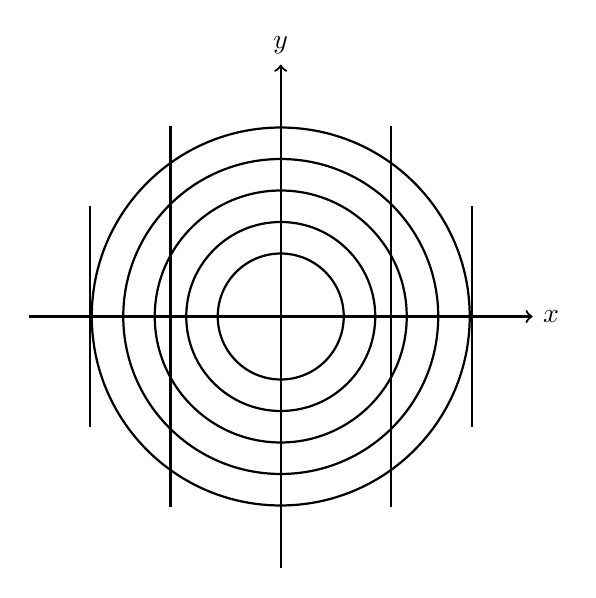
\begin{tikzpicture}[scale=0.8]
            % Concentric circles
            \foreach \r in {1, 1.5, 2, 2.5, 3} {
                \draw[thick] (0,0) circle (\r);
            }
            % Orthogonal lines
a one-parameter            \foreach \a in {0, 30, 60, 90, 120, 150} {
                \draw[thick] (-\a:3.5) -- (\a:3.5);
                \draw[thick] (-\a+180:3.5) -- (\a+180:3.5);
            }
            % Axes
            \draw[->, thick] (-4,0) -- (4,0) node[right] {$x$};
            \draw[->, thick] (0,-4) -- (0,4) node[above] {$y$};
        \end{tikzpicture}
    \end{center}
\end{tcolorbox}

\begin{tcolorbox}[colback=LightBg, colframe=BorderGray, arc=4mm]
    {\small\textbf{\textcolor{AccentBlue}{EXAMPLE: ORTHOGONAL TRAJECTORIES}}}
    \vspace{0.2cm}\\
    \textbf{Find the orthogonal trajectories of $y = cx^2$}
    
    \vspace{0.2cm}
    \textbf{Solution:} \\
    Differentiating $\implies \displaystyle \frac{dy}{dx} = 2cx = 2 \left(\frac{y}{x^2}\right) \cdot x = \frac{2y}{x}$ \\
    Replacing $\frac{dy}{dx}$ by $-\frac{dx}{dy}$ we get,
    \[ -\frac{dx}{dy} = \frac{2y}{x} \]
    which is the DE of orthogonal trajectory $\implies 2y dy + x dx = 0$.
    
    Integrating, $y^2 + \frac{x^2}{2} = k_0 \implies$ (Separating the vars) \\
    $\implies 2y^2 + x^2 = 2k_0 = k^2$ \\
    which is the family of orthogonal trajectories of the given family $y = cx^2$.
\end{tcolorbox}

\begin{tcolorbox}[colback=LightBg, colframe=BorderGray, arc=4mm]
    {\small\textbf{\textcolor{AccentBlue}{EXAMPLE: OBLIQUE TRAJECTORIES}}}
    \vspace{0.2cm}\\
    \textbf{Find a family of oblique trajectories of the family of straight lines $y = cx$ at angle $\alpha = 45^\circ$.} (S.L. Ross p75)
\end{tcolorbox}

\section{Higher Order Linear DE}
A LODE (Linear Ordinary Differential Equation) of order $n$ in the dependent variable $y$ and the independent variable $x$ is an equation that can be expressed in the form, 
\begin{equation}
    a_0(x)\frac{d^ny}{dx^n} + a_1(x)\frac{d^{n-1}y}{dx^{n-1}} + \dots + a_{n-1}(x)\frac{dy}{dx} + a_n(x)y = F(x)
\end{equation}
where $a_0(x) \neq 0$.

We shall assume that $a_0, a_1, \dots, a_n$ are continuous on an interval $a \leq x \leq b$ \& $a_0 \neq 0$ $\forall x$ on $a \leq x \leq b$. \\
The right-hand member $F(x)$ is called the \ textbf {non-homogeneous} term. \\
If $F(x) = 0$ then eqn (1) reduces to:
\begin{equation}
    a_0(x)\frac{d^ny}{dx^n} + a_1(x)\frac{d^{n-1}y}{dx^{n-1}} + \dots + a_{n-1}(x)\frac{dy}{dx} + a_n(x)y = 0
\end{equation}
and is then called \textbf{homogeneous}.

Let $x_0$ be any point on $a \leq x \leq b$ and let $c_0, c_1, \dots, c_{n-1}$ be arbitrary constants of $n$. \\
There exists a unique solution $f^*$ of Eqn (1) s.t.
\[ f(x_0) = c_0, \ f'(x_0) = c_1, \ \dots, \ f^{(n-1)}(x_0) = c_{n-1} \]
which is defined on $a \leq x \leq b$.

\textbf{Note:} Let $f$ be a solution of (2) then $f(x_0) = 0, f'(x_0) = 0, \dots, f^{(n-1)}(x_0) = 0$.

\end{document}
